% Created 2020-12-11 sex 18:54
% Intended LaTeX compiler: pdflatex
\documentclass[11pt]{article}
\usepackage[utf8]{inputenc}
\usepackage{lmodern}
\usepackage[T1]{fontenc}
\usepackage[top=3cm, bottom=2cm, left=3cm, right=2cm]{geometry}
\usepackage{graphicx}
\usepackage{longtable}
\usepackage{float}
\usepackage{wrapfig}
\usepackage{rotating}
\usepackage[normalem]{ulem}
\usepackage{amsmath}
\usepackage{textcomp}
\usepackage{marvosym}
\usepackage{wasysym}
\usepackage{amssymb}
\usepackage{amsmath}
\usepackage[theorems, skins]{tcolorbox}
\usepackage[style=abnt,noslsn,extrayear,uniquename=init,giveninits,justify,sccite,
scbib,repeattitles,doi=false,isbn=false,url=false,maxcitenames=2,
natbib=true,backend=biber]{biblatex}
\usepackage{url}
\usepackage[cache=false]{minted}
\usepackage[linktocpage,pdfstartview=FitH,colorlinks,
linkcolor=blue,anchorcolor=blue,
citecolor=blue,filecolor=blue,menucolor=blue,urlcolor=blue]{hyperref}
\usepackage{attachfile}
\usepackage{setspace}
\usepackage{tikz}
\addbibresource{refs.bib}
\usepackage{svg, caption, multirow, booktabs}
\usepackage[english]{babel}
\author{Gabriel Petrini, Lucas Teixeira}
\date{\today}
\title{Long-run effective demand and residential investment: a Sraffian supermultiplier based analysis}
\begin{document}

\maketitle
\begin{abstract}
In this paper, we build a fully specified parsimonious Sraffian supermultiplier stock-flow consistent model (SSM-SFC) with two non-capacity creating autonomous expenditure: residential investment and debt-financed consumption.
Our model represents a closed and without government economy with workers and capitalist households and only the latter are not credit constrained.
The introduction of residential investment implies that our SSM-SFC model has two real assets: firms' productive capital and households' real estate.
In our model, residential investment growth rate responds to changes of house price inflation.
The numerical simulation experiments shows that our model keep the main standard Sraffian supermultiplier growth models results.
As a particular result, an increase of residential investment growth rate increase implies a decrease of real estate share in total real assets.
Inspired by the recent U.S. bubble episode, we plug house price inflation data (1992-2019).
Although simple, our numerical simulations are capable to reproduce some stylized facts such as residential investment leading the business cycle and capital accumulation and a clockwise pattern between non-capacity creating autonomous expenditures and capacity utilization rate.

\noindent \textbf{Keywords:} Residential Investment; Sraffian supermultiplier; Asset bubble;  Stock-Flow Consistent approach.
\end{abstract}


\section{Introduction}
\label{sec:org8c1ea9b}
\label{sec:introduction}
Non-residential investment is the most scrutinized variable in demand-led growth models so that others expenditures are given a secondary role \cite{brochier_macroeconomics_2017}.
More than a decade after the Great Recession, this is still the case for residential investment which continues to receive sparse and unsystematic attention by the literature \cites{caverzasi_stock-flow_2013}{nikolaidi_minsky_2017}.
Despite its absence in theoretical models, there is a growing empirical literature highlighting its macrodynamic relevance \cites{leamer_housing_2007}{jorda_great_2014}{fiebiger_semi-autonomous_2018}{fiebiger_trend_2017}.


Sraffian supermultiplier growth model (SSM) establishes an important role to non-capacity creating (NCC) autonomous expenditures such
as residential investment.
\textcite{serrano_long_1995,serrano_sraffian_2017} present a simple version of the SSM model to highlight it as an alternative closure for heterodox growth theory.
More recently, \textcites{allain_tackling_2015}{lavoie_post-keynesian_2015}{lavoie_convergence_2016} have introduced SSM to a broader Post-Keynesian audience.

Different NCC autonomous expenditures have been included in this framework. 
For instance, some scholars have investigated the macroeconomic implications of both debt-financed \cites{pariboni_autonomous_2015}{fagundes_role_2017}{mandarino-2020-worker-debt} and financial wealth-financed consumption \cite{brochier_supermultiplier_2018}.
The same applies to government expenditures \cites{allain_tackling_2015}{bougrine_autonomous_2020} and exports \cite{nah_long-run_2017}.

Even though these works emphasize the relevance of some NCC autonomous expenditures, residential investment has received little attention.
\textcites{zezza_u.s._2008}{nikolaidi_securitisation_2015} include residential investment in a SFC model with others objectives than its implications to economic growth and business cycles.
In a recent contribution, \textcite{dejuan_supermultiplier-cum-finance_2018} present an SSM model with residential investment.
They build a model in order to analyze the destabilizing effects of household over-indebtedness without exploring the determinants of residential investment.

This paper is a first step in building the connection between house price inflation and residential investment.
In order to do so, we build a fully specified parsimonious Sraffian supermultiplier stock-flow consistent model (SSM-SFC) with residential investment.

The remainder of this paper is organized as follows.
Section \ref{sec:empirical} discuss some residential investment related stylized facts for the US economy related to house bubble, residential investment and its macroeconomic implications.
Section \ref{sec:Model} presents a SSM-SFC model  with asset bubbles and two real assets: firms' capital and household' real estate. 
Section \ref{sec:runs} evaluates short-, traverse and long-run equilibria in order to access the consequences of residential investment inclusion on output level and growth and stock-flow ratios.
Next, Section \ref{sec:Experiments} evaluates this relations through numerical simulations.
Inspired by the recent housing bubble episode, the experiments are: decrease in wage-share (Section \ref{sec:Exp1}); increase in real estate inflation (Section \ref{sec:Exp2}); and an increase in interest rate \ref{sec:Exp3}).
In this same Section, we also plug houses own rate of interest observed data for the U.S. (from 1992 to 2019) in order to compare simulations' results with the stylized facts presented previously.
Section \ref{sec:Conclusion} offers some concluding remarks while Appendix \ref{append:Data} provides simulation's parameters and baseline values.



\section{Empirical Motivation}
\label{sec:org8990bf3}
\label{sec:empirical}
A growing body of empirical demand-led literature has evaluated the role of NCC autonomous expenditures.
\textcite{freitas_pattern_2013} present a growth accounting decomposition fro Brazil from 1970 to 2005 and report the relevance of those expenditures in describing Brazilian GDP growth. \textcite{braga_investment_2018} shows evidence that economic growth and non-residential investment are explained by NCC autonomous expenditures in Brazilian economy from 1962 to 2015. For the U.S., \textcite{girardi_long-run_2016} show that NCC autonomous expenditures have permanent effects on growth rate. 
\textcite{haluska_growth_2019} employ Granger-causality tests to assess the stability of the SSM for the US (1987-2017) and report a causality from NCC autonomous expenditures to the marginal propensity to invest, as expected.
Finally, \textcite{girardi_autonomous_2018} bring evidence that those expenditures determine investment share on GDP for twenty OECD countries.

\\
However, there still is a lack of studies on the role of residential investment specifically.
What is commonly  discussed about this NCC autonomous expenditure is largely based on \textcite{green_follow_1997} pioneer work.
Based on Granger Causality and cointegration tests for the US from 1959-1992, this is one of the first papers to indicates that residential investment leads the business cycle.
Subsequently, \textcite{leamer_housing_2007} concludes that this pattern occurs at least since the post-war period.
More precisely,  \textcite[p.~8]{leamer_housing_2007} describes US business cycles as follows: ``[f]irst homes, then cars,
and last business equipment''.
Recently, \textcites{fiebiger_semi-autonomous_2018}{fiebiger_trend_2017} also report residential investment as an important determinant of business cycles for the US based on causal narratives.
Alternatively, \textcite{huang_is_2020} estimate a Structural Vector Autoregressive (SVEC) model in a time-scale framework for the OECD countries to assess both prediction and causality relations stated by \textcite{leamer_housing_2007}.
They report that residential investment predicts the US  macroeconomic fluctuation and housing related variables (house prices, real mortgage rate --- deflated by a general price index --- and bank spread) lead the business cycle in all G7 countries.

\\
After the Great Recession (2008-2009), there has been growing macroeconometric studies on housing.
However, most of them have emphasized house prices and not its volume (residential investment).
\textcite{goodhart_house_2008} for instance, estimate a time-series fixed effects panel data for 17 industrialized countries from 1970 to 2006. They report a multidirectional relation between money, credit, house prices and GDP growth and have found stronger effects during housing booms\footnote{\textcite{Arestis_Bank_2014} also found a  direct relationship between house prices and credit volume based on cointegration and error correction techniques for 9 OECD countries from 1970 to 2011.}. 
\textcite{wood_house_2020} report that house prices are relevant for describing household indebtedness from 1980 to 2017 in 18 advance economies.
However, both studies do not include residential investment.
\textcite{arestis_residential_2015}, on the other side, include residential investment. Using a ARDL model for 17 OECD countries from 1970 to 2013, the authors report that banking credit and real house prices are the most statistically significant variables for real residential investment in the US.
Although those approaches are interesting, it fails to take into account the connection between asset bubbles and aggregate demand which is relevant for describe the recent housing burst event.

\\
From this review of recent empirical literature, it is noticeable that few macroeconometric studies have investigated residential investment in any systematic way.
In this paper, we argue that besides this growing body of literature that recognizes the macroeconomic importance of residential investment, little progress has been made in connecting asset bubbles with its macroeconomics consequences.
On the following subsection, we present some residential investment-related stylized facts in order to highlight its relevance for the US business cycle which will be compared to the theoretical model in Section \ref{real_sim}.
Next, we analyze the connection between residential investment, real estate inflation and mortgage interest rate during the U.S. housing bubble episode.

\subsection{Residential investment stylized facts}
\label{sec:orgbf10484}

As discussed before, both \textcites{green_follow_1997}{leamer_housing_2007} made it clear how important this particular expenditure is to USA business cycle. In this subsection, we show some residential investment stylized facts for the US in more detail.

\begin{itemize}
\item[{$\square$}] Introdução mais alongada
\end{itemize}

Figure \ref{Investo_Resid_GDP} shows how residential investment movements help to predict recessions. Recessions are anticipated by a reduction of residential investment share on GDP, while the expansion of those expenditures precedes economic recovery. The fall of dwellings expenditures in 1966-67 are an exception because the increase of military expenditures because of Vietnam War offset an eventual economic downturn \cite[p.~20]{leamer_housing_2007}. Another exception is the dot-com bubble 2000 crisis that was not caused by residential investment. The Great Recession 2008-2009 is the one in which this pattern is the most evident. 



\begin{figure}[htb]
    \centering
        \caption{Residential Investment as share of GDP}
        \label{Investo_Resid_GDP}
    \includegraphics[width = 0.7\textwidth]{./figs/res_share.png}
    \caption*{\textbf{Source:} Federal Reserve Bank of St. Louis, authors’ elaboration}
\end{figure}

In order to depict the relation between housing and business cycle, we present Figure \ref{fig:cycles} in which each cycle is represented in a different panel\footnote{Similar reasoning can be found in \textcite{fiebiger_trend_2017}. Unlike them, we plot only residential investment without including other households expenses financed by credit.}.
Residential investment-GDP ratio and capacity utilization --- as a proxy for business cycle --- are presented on vertical and horizontal axis respectively.
Economic recovery is generally characterized by residential investment growing faster than GDP\footnote{It worth noting that 1991-2000 period is a particular case.}. Both residential investment share on GDP and capacity utilization increase as a consequence of higher residential investment growth rate.
Accordingly to the Sraffian Supermultiplier model, we can interpret subsequent non-residential investment increase as a result of capital stock adjustment principle. 
This increase implies GDP to grow faster than residential investment, therefore reducing both its share on GDP and capacity utilization ratio. Finally, as a result of economic burst, capacity utilization ratio falls and the cycle ends.



\begin{figure}[htb]
    \centering
        \caption{Share of residential investment and capacity utilization during business cycles\\\centering (Dots size grow in  time)} 
    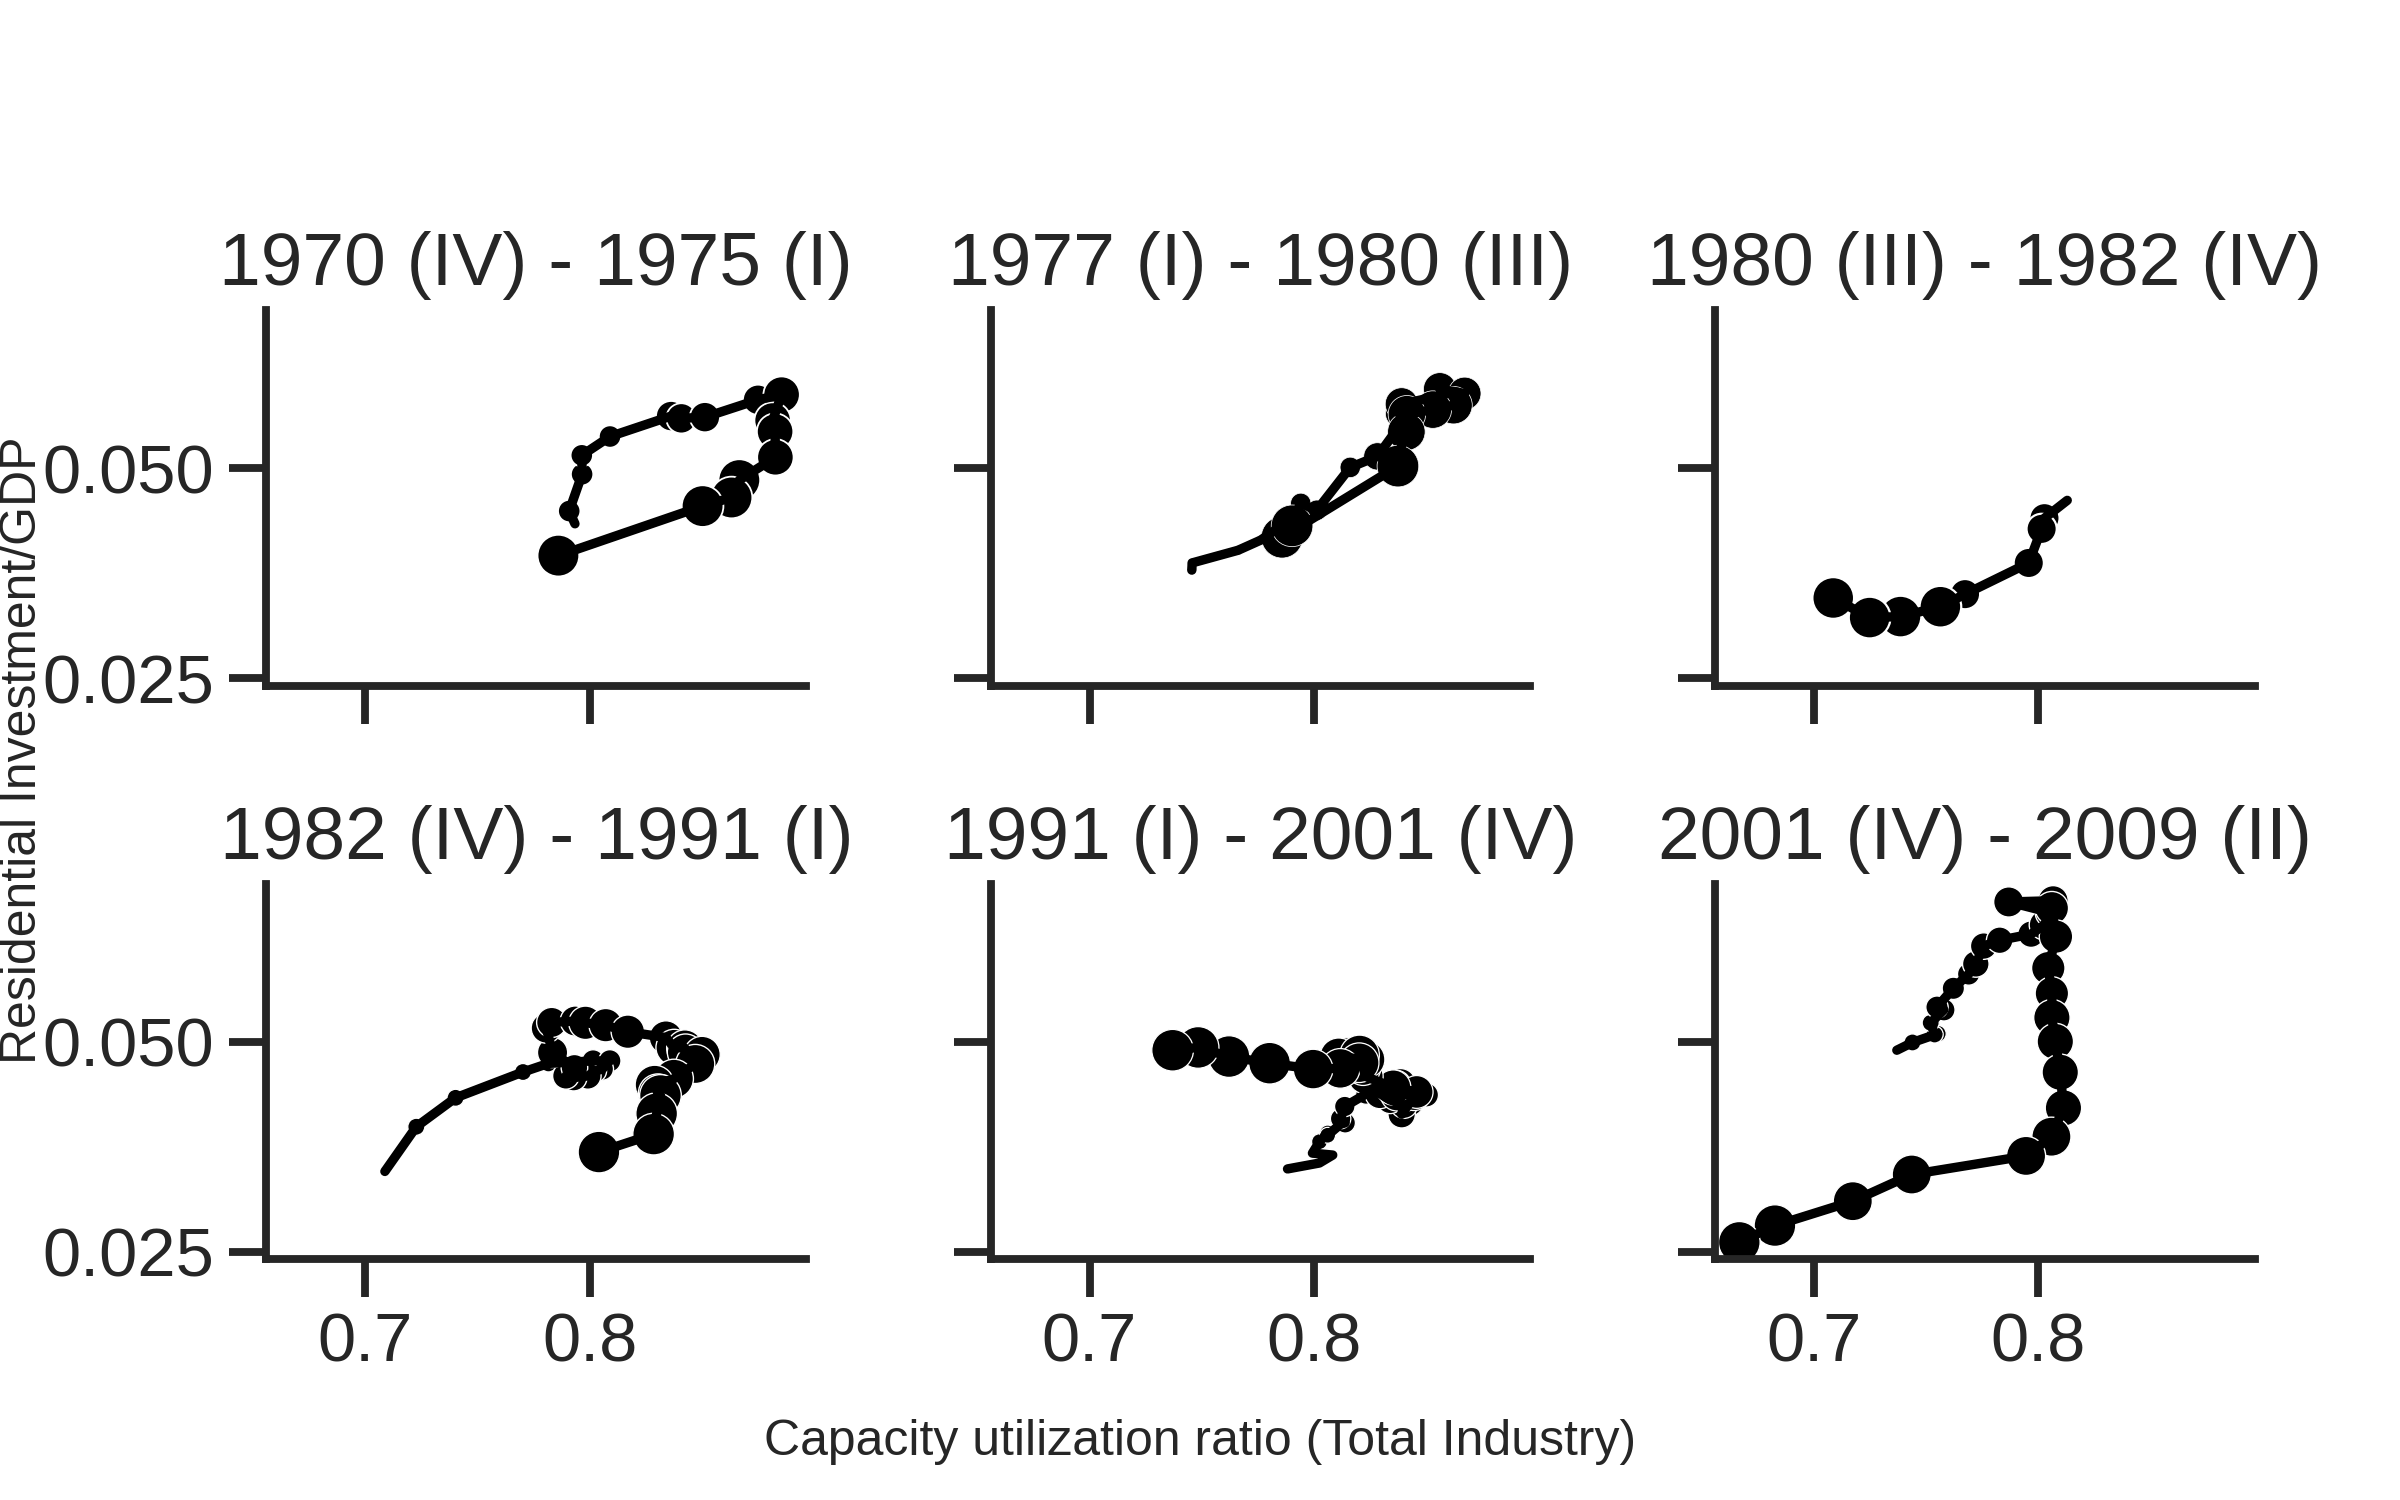
\includegraphics[width = 0.9\textwidth]{./figs/cycles.png}
    \label{fig:cycles}
    \caption*{\textbf{Source:} Federal Reserve Bank of St. Louis, authors’ elaboration.}
\end{figure}

\subsection{Housing bubble and residential investment}
\label{sec:org473bac1}
Once residential investment is relevant to describe the U.S. business cycle, it is important to understand its determinants.
There are at some key variables to assess the residential investment behavior.
The first variable is the mortgage interest rate, which determines the financial cost of buying houses and the weight of debt-service on house investors' income.
The other is rate of change house prices.
The one who owns a house or is willing to buy one takes into consideration the change of the asset price.
This happens because of speculative reasons or just to prevent capital loss and reductions of net worth.

Based on \citeauthor*{Sraffa_Own_1932}'s \citeyear{Sraffa_Own_1932} commodity rate of interest, \textcite{teixeira_crescimento_2015} proposes the so-called houses own rate of interest.
Estimated by deflating mortgages interest rate real estate inflation, this particular real interest rate is the most relevant for house buyers since it is the real cost in real estate from buying real estate  \cite[p.~53]{teixeira_crescimento_2015}.
This particular interest rate is shown in Equation \ref{_own} in which \(own\) stands for houses own rate of interst, \(r_{mo}\) for mortgage interest rate and \(\pi\) for house price inflation.


\begin{equation}
\label{_own}
own = \left(\frac{1+r_{mo}}{1+\pi}\right) -1
\end{equation}

During a housing bubble period, it is real estate inflation that governs own's interest rate movements. Therefore, the lower this rate is, the greater the capital gains (in real estate) for speculating with real estate will be. This negative relation between houses own interest rate and residential investment is shown in Figure \ref{propria_investo} in which this particular real interest rate has been gradually decreased over the real estate boom (2002-5).
Additionally, Figure \ref{propria_investo} illustrates how this  procedure is more adequate than a consumer price index deflation --- as \textcite[p.~143--6]{fair_macroeconometric_2013} does --- to describe residential investment growth rate\footnote{Based on this concept, \textcite{petrini_demanda_2019} estimated time series econometric model for the U.S. (1992 to 2019) and presents empirical evidence that residential investment growth rate and houses own rate of interest hare a common negative long-run trend.  Furthermore, \textcite{petrini_demanda_2019} also reports a unidirectional long-run causality from houses own rate of interest to residential investment growth rate.}.


\begin{figure}[htb]
	\centering
	\caption{Residential investment growth rate vs. Houses Own interest rate}
	\label{propria_investo}
	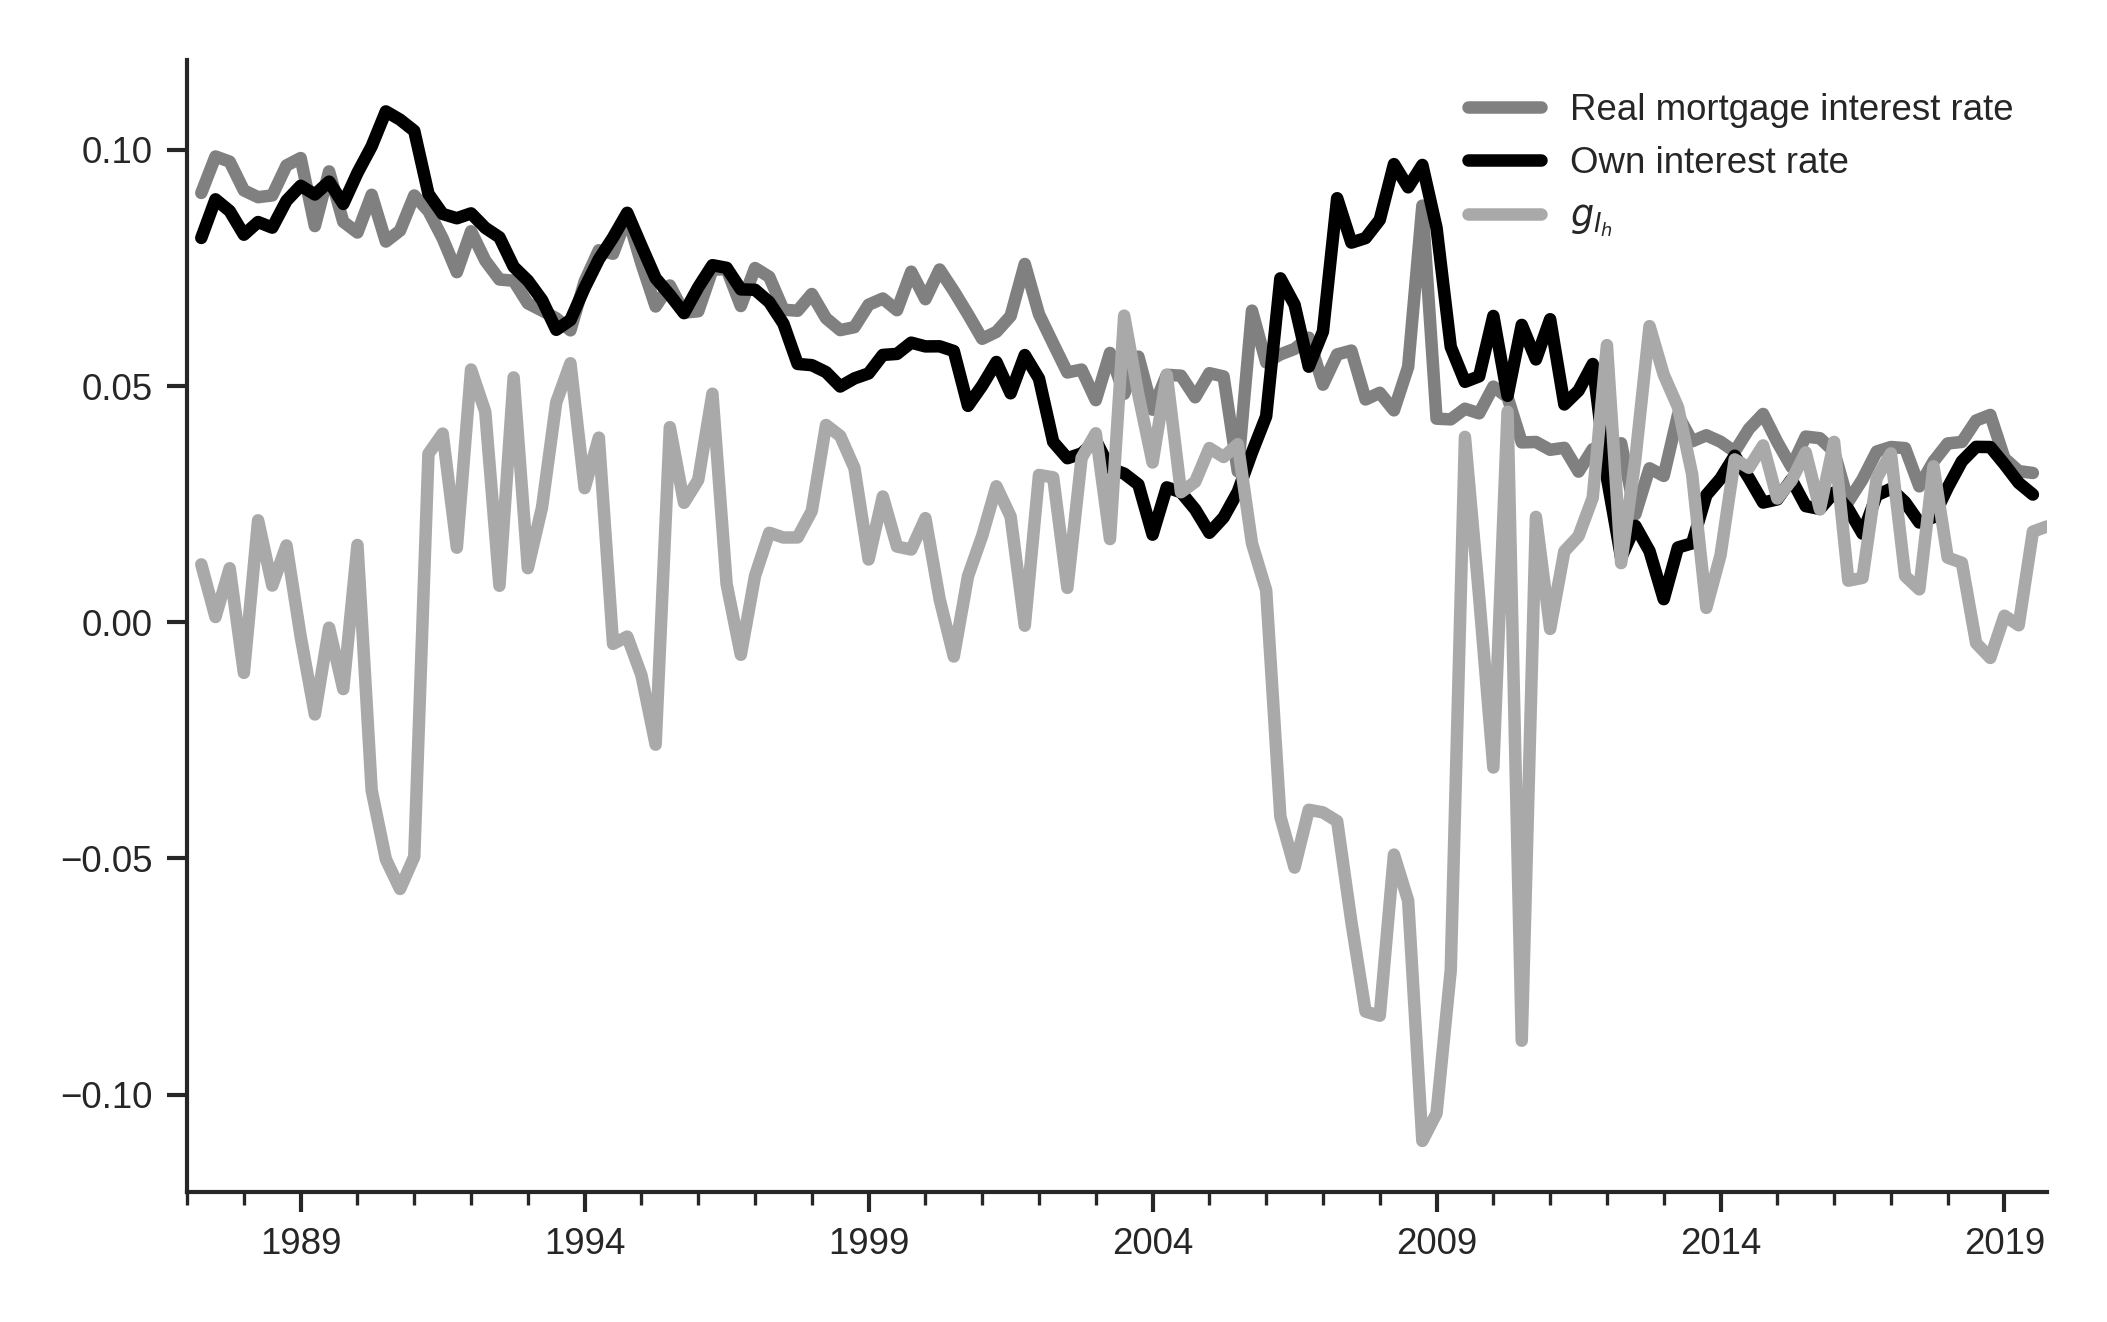
\includegraphics[width=.8\textwidth]{./figs/Own_gI}
	\caption*{\textbf{Source:} U.S. Bureau of Economic Analysis, Authors' elaboration}
\end{figure}


In summary, we presented some stylized facts that highlights the relevance of residential investment for the U.S. business cycle and the relevance of house bubbles to the residential investment.
In the next section, we build a fully specified parsimonious Sraffian supermultiplier stock-flow consistent model (SSM-SFC) to deal with these stylized facts.


\section{A Sraffian supermultiplier SFC model with residential investment}
\label{sec:org4924ada}
\label{sec:Model}
\subsection{General equations}
\label{sec:org8ed2384}

Our model is the most parsimonious as possible: a closed capitalist economy without government sector. Output (\(Y\)) is determined by  a fixed combination of a homogeneous labor (\(L\)) input with homogeneous fixed business capital (\(K_f\)). 
For simplicity, we put technological progress, depreciation and goods inflation aside so investment is presented in net terms and all variables --- except for houses --- are measured in real terms.
Assuming a Leontief production function and that growth is not constrained by labor scarcity, full capacity output (\(Y_{FC}\)) is
determined by firms' capital stock:
\begin{equation}
\label{_Leontieff}
    Y_{FC} = \min (Y_L, Y_K)
\end{equation}
\begin{equation}
\label{_YFC}
    Y_{FC} = \frac{K_{f_{-1}}}{v}
\end{equation}
\begin{equation}
\label{_u}
    u = \frac{Y}{Y_{FC}}
\end{equation}
where \(Y_L\) and \(Y_K\) stands for full employment and full capacity output respectively, \(v\) is exogenous capital-output ratio and \(u\) is utilization rate.

We further assume an economic structure composed by both workers (denoted by subscript \(w\)) and capitalists (denoted by subscript \(k\)) households.
Thus, demand-determined output level (\(Y\))  is the sum of workers and capitalists consumption (\(C_w\) and \(C_k\) respectively) and both households and firms investment (\(I_h\) and \(I_f\) respectively) and only the latter creates capacity to the business sector of the economy:
\begin{equation}
\label{_Ct}
    C = C_w + C_k
\end{equation}
\begin{equation}
\label{_It}
    I_t = I_f + I_h
\end{equation}
\begin{equation}
\label{_Y}
    Y = \overbrace{[C_w + \underbrace{C_k + I_h}_{\text{Capitalists}}]}^{\text{Households}} + \overbrace{[I_f]}^{\text{Firms}}
\end{equation}

In other words, from institutional sectors perspective, household expenditures have two components (consumption and residential investment) and firms just one (non-residential investment).
So, the novelty of this model is the inclusion of a second investment component all made by household sector and held by capitalists households for simplicity. 
Therefore, this economy produces two types of real assets: firms productive capital (\(K_f\)) and households housing (\(K_h\)):
\begin{equation}
    \label{_K}
    K = K_f + K_h
\end{equation}

Denoting the houses share in total real assets as \(k\), we can rewrite equation \ref{_K} as:
\begin{equation}
\label{_k}
    k = \frac{K_h}{K}
\end{equation}
$$
K = (1-k)\cdot K + k\cdot K
$$

Following Sraffian literature, functional income distribution is determined both by historical-institutional factors and class struggle. 
As consequence, wage-share (\(\omega\)) is considered exogenous to out model and define total wages as (\(W\), Eq. \ref{_W}): 

\begin{equation}
\label{_W}
    W = \omega\cdot Y
\end{equation}

Table \ref{Matriz_Estoques} presents the balance sheet matrix for all institutional sectors. 
Capitalists households hold financial wealth as bank deposits (\(M\)) and residential investment is financed by mortgages (\(MO\)).
Capitalists' total net wealth (\(NW_{k}\)) is the sum of their net financial wealth (\(V_{k}\)) and real assets (\textit{i.e.} housing, \(K_h\)). 
Table  \ref{Matriz_Fluxos} presents both transactions flows and the flow of funds matrix. 
This table shows all economic relations between institutional sectors ensuring that there is no  ``black holes''
so all financial and real transaction are explicitly defined \cite{macedo_e_silva_peering_2011}.

In this model, capitalist consumption (\(C_k\)) is fully autonomous and financed by loans (\(L_{k}\)) while workers consumption (\(C_w\)) is fully induced by their wages.
We assume that workers expend what they earn while capitalists earn what they expend, so workers financial and real wealth are both null.
Firms finance their investment primarily by undistributed profits (\(FU\)) and the residual by bank loans (\(L_f\)) --- thus they do not hold deposits. 
Banks create credit \textit{ex nihilo} and then collect the deposits, paying the same interest rate that they charge.
On the following subsections, we will present the equations of each of these institutional sectors.



\begin{table}[H]
\centering
\caption{Balance Sheet matrix}
\label{Matriz_Estoques}
\begin{tabular}{lccccc}
\hline
\hline
                          & Workers & Capitalists      & Firms        & Banks  &    $\sum$ \\ \hline

Deposits & & $+M$ & & $-M$ & 0\\
Loans& &$-L_{k}$ &$-L_f$& $+L$ & 0\\
Mortages & &$-MO$&  & $+MO$ & 0\\\hline
$\sum$ Net Financial Wealth &--- &$V_{k}$&$V_f$&$V_b$& $0$\\\hline
Capital & & &$+K_f$&  & $+K_f$\\
Houses & &$+K_{hd}$& &   & $+K_h$\\\hline
$\sum$ Net Wealth &---&$NW_{k}$&$NW_f$&$NW_b$& $+K$\\
\hline
\hline
\end{tabular}%
\caption*{\textbf{Source:} Authors' Elaboration}
\end{table}


\begin{table}[H]
\centering
\caption{Transactions flow matrix and flow of funds
}
\label{Matriz_Fluxos}
\resizebox{\textwidth}{!}{%
\begin{tabular}{lccccccc}
\hline
\hline
& Workers
& \multicolumn{2}{c}{Capitalists}
& \multicolumn{2}{c}{Firms}                        
& Banks       & Total    \\ \cline{3-4}\cline{5-6}
& &
Current & Capital & 
Current & Capital     & 
&       $\sum$ \\ 
Consumption                       &$-Cw$&$-C_k$& & $+C$& & & 0\\
Non-residential Investment                   & & & &$+I_f$&$-I_f$ & & 0\\
Residential Investment       &  & &$-I_h$&$+I_h$& & & 0\\
\textbf{{[}Output{]}}   & & & &{[}$Y${]}& & & {[}$Y${]}\\
Wages                        &$+W$&& &$-W$& & & 0\\
Profits                      & &$+FD$& &$-FT$&$+FU$& & 0\\
Deposits interest rate         & &$+r_m\cdot M_{-1}$& && &$-r_m\cdot M_{-1}$& 0\\
Loans interest rate         & &$-r_l\cdot L_{k_{-1}}$& &$-r_l\cdot L_{f_{-1}}$& &$+r_l\cdot L_{-1}$& 0\\

Mortages interest rates         & &$-r_{mo}\cdot MO_{-1}$& && &$+r_{mo}\cdot MO_{-1}$& 0\\\hline
\textbf{Subtotal}           &---&$+S_h$&$-I_h$& &$+NFW_f$&$+NFW_b$& 0\\\hline
Change in deposits     & &$-\Delta M$& & & &$+\Delta M$& 0\\
Change in mortgages     & & &$+ \Delta MO$& & &$-\Delta MO$& 0\\
Change in loans     & &$+\Delta L_{k}$&&$+\Delta L_f$& &$-\Delta L$& 0\\
\textbf{Total} & & 0 & 0 & 0  & 0  & 0  & 0\\
\hline
\hline
\end{tabular}%
}
\caption*{\textbf{Source:} Authors' Elaboration}
\end{table}


\subsection{Firms}
\label{sec:org9fdd3e2}

In order to produce, firms purchase capital goods (\(-I_f\) in capital account) and hire workers, whom total remuneration is the economy wage bill. 
Their total profits (\(FT\)) are a residual between sales (\(Y\)) and total wages (\(W\)). 
Firms retain part (\(\gamma_F\)) of profits net of interest payments (\(FU\)) --- to reinvest --- and distribute the rest to capitalists (\(FD\)):

\begin{equation}
\label{_FT}
    FT = Y - W = FD + FU
\end{equation}
\begin{equation}
    FU = \gamma_F\cdot (FT - r_l\cdot L_{f_{-1}})
\end{equation}
\begin{equation}
    FD = (1-\gamma_F)\cdot (FT - r_l\cdot L_{f_{-1}})
\end{equation}

Firms (non-residential) investment is fully induced by the level of effective demand (Eq. \ref{_If}), and its growth rate changes accordingly to the capital stock adjustment principle \cite{freitas_growth_2015}.
Equation \ref{_h} in one simple way to describe this mechanism.
According to it, the marginal propensity to invest (\(h\)) endogenously adjust to discrepancies between actual and normal utilization rates (\(u\) and \(u_N\), respectively). 
For this mechanism to take place, the adjustment parameter (\(\gamma_u\)) must be sufficiently small and non-negative\footnote{The size of this parameter guards a fundamental relation to the stability of the model, as shown by \textcite{freitas_growth_2015}.}. 
As a consequence, productive capacity gradually adjusts to effective demand movements.

\begin{equation}
\label{_If}
    I_f = h_{t-1}\cdot Y
\end{equation}
\begin{equation}
\label{_h}
    \Delta h = h_{t-1}\cdot \gamma_u\cdot (u - u_N)
\end{equation}
\begin{equation}
    \Delta K_f = I_f
\end{equation}


Firms finance part of investment that exceeds undistributed profits by bank loans, paying an interest rate on it (\(r_l\)) charged by the banks. 
We assume an elastic supply of credit for investment. 
Moreover, tables \ref{Matriz_Estoques} and \ref{Matriz_Fluxos} show firms net wealth (\(NW_f\)) and net financial balance (\(NFW_f\)) explicitly:

\begin{equation}
\label{_Lf}
    \Delta L_f = I_f - FU
\end{equation}
\begin{equation}
\label{_rg}
r_g = \frac{(1-\omega)\cdot u}{v}
\end{equation}
\begin{equation}
\label{_rn}
r_n = r_g - r_l\cdot\frac{L_{f_{-1}}}{K_f}
\end{equation}
\begin{equation}
    NFW_f = FU - I_f
\end{equation}
\begin{equation}
    NW_f = K_f - L_f
\end{equation}
where \(r_g\) and \(r_n\) denotes gross and net profit rate respectively.

\subsection{Banks}
\label{sec:orgcb2c814}

As in most part of SFC literature, banks do not have an active role in this model.
They create money as credit is demanded and just after they collect deposits \cite{le_bourva_money_1992}. 
Firms finance part of their investment with credit (\(L_f\)) and capitalists households finance all their residential investment by mortgages (\(MO\)) and consumption by loans (\(L_{k}\)), as already mentioned.
For simplicity, we assume null bank spreads (\(\sigma_{mo} = \sigma_l = 0\)) so interest rate on mortgages (\(r_{mo}\)) and on loans (\(r_{l}\))
are the same as on deposits (\(r_{m}\)) which is  exogenously determined by banks.
Banks net balances (\(NFW_b\)) are defined by interests received net of interests payments. 
As those interests are the same, banks net wealth is necessarily zero (see table \ref{Matriz_Estoques}) and deposits are residuum:

\begin{equation}
L = L_f + L_{k}
\end{equation}
\begin{equation}
    r_l = (1+\sigma_l)\cdot r_m
\end{equation}
\begin{equation}
    r_{mo} = (1+\sigma_{mo})\cdot r_m
\end{equation}
\begin{equation}
    r_m = \overline r_m
\end{equation}
\begin{equation}
    NFW_b = r_{mo}\cdot MO_{-1} + r_l\cdot L_{-1} - r_m\cdot M_{-1}
\end{equation}
$$
NFW_b = \Delta MO + \Delta L - \Delta M
$$
\begin{equation}
    NW_b = V_b \equiv 0
\end{equation}
\begin{equation}
\label{_M}
    \Delta M = \Delta L + \Delta MO
\end{equation}

\subsection{Households}
\label{sec:org9ac1da9}

\subsubsection*{Workers}
\label{sec:org1bd83c3}
As mentioned before, we assume that workers expend (\(C_w\)) what they earn (\(W\)). 
For simplicity, we consider that wages are the only source of income workers' disposable income (\(YD_{w}\)) and do not have access to consumption loans, so worker' saving (\(S_{hw}\)) are null.
Therefore, accordingly to our hypothesis, workers' do not hold both net financial and total wealth (\(V_{w}\)).

\begin{equation}
C_w = W
\end{equation}
\begin{equation}
YD_w = W
\end{equation}
\begin{equation}
S_{w} = YD_w - C_w
\end{equation}
$$
S_{w} = 0
$$
\begin{equation}
NFW_{w} = S_{w} = 0
\end{equation}
\begin{equation}
V_{w} = 0
\end{equation}

\subsubsection*{Capitalists}
\label{sec:org0e5e5c0}
This is the most complex institutional sector of our model. 
We assume consumption (\(C_k\)) is fully-autonomous and financed by loans (\(L_{k}\)). 
Disposable income (\(YD_k\)) is the sum of distributed profits and received interests on deposits, net of interests payments
on both mortgages and loans.
Capitalists savings (\(S_{k}\)) are disposable income net of consumption.
At odds with SFC literature, savings are not equal to net balance (\(NFW_{k}\)) since we have included residential investment as in Equation \ref{NFWh}.

\begin{equation}
\Delta L_{k} = C_k
\end{equation}
\begin{equation}
    \label{EqYD}
    YD_k = FD + \overline r_m\cdot M_{-1} - r_{mo}\cdot MO_{-1} - r_{l}\cdot L_{k_{-1}}
\end{equation}
\begin{equation}
    \label{EqSh}
    S_{k} = YD_k - C_k
\end{equation}
\begin{equation}
\label{NFWh}
    NFW_{k} = S_{k} - I_h
\end{equation}


As mentioned before, capitalist households are the only institutional section investing in houses which is financed by mortgages as in equation (\ref{EqMO}). 
Thus, capitalists' total debt stock (\(D\)) is sum of mortgage and consumption loans (Equation \ref{k_D})

\begin{equation}
  \label{EqMO}
  \Delta MO = I_h
\end{equation}
\begin{equation}
  \label{k_D}
  D =  MO + L_k
\end{equation}



Next, we present residential investment growth rate (\(g_{I_h}\)) as determined by houses own rate of interest (\(own\), equation \ref{_own}) as introduced by \textcite{teixeira_crescimento_2015} and discussed in section \ref{sec:empirical}.


\begin{equation}
    I_h = (1 + g_{I_h})\cdot Ih_{-1}
\end{equation}
\begin{equation}
\label{g_Z_own}
g_{I_h} = \phi_0 - \phi_1\cdot own
\end{equation}
where  \(\phi_0\) represents long-term determinants of residential investment (\emph{e.g.} demographic factors, housing and credit policies, etc.)\footnote{For an early discussion about long-term determinants of residential investment see \textcite{grebler_capital_1956}. For a historical-institutional discussing of mortgage markets, see \textcite{green_american_2005}.} while \(\phi_1\) captures the demand for housing arising from expectations of capital gains resulting from speculation with flow of new houses. 

Accordingly to our hypothesis, nominal (\(V_{nk}\)) and real net wealth (\(V_{k}\)) are distinguished only by the inclusion of real estate price (\(p_h\)) and are defined as follows:
\begin{equation}
V_{k} = K_{hd} + M - L_{k} - MO
\end{equation}
\begin{equation}
V_{nk} = K_{hd}\cdot p_h + M - L_{k} - MO
\end{equation}


In order to fulfill our goals, we employ \citeauthor*{freitas_baseline_2020}'s \citeyear{freitas_baseline_2020} procedure in which NCC autonomous expenditure (\(Z\)) composition (\(R\)) remains unchanged. Thus, we can express capitalists total consumption as follows:

\begin{equation}
\label{_Z}
Z = C_k + I_h
\end{equation}
$$
\frac{C_k}{Z} + \frac{I_h}{Z} = R + (1-R)
$$
which allows us to rewrite both residential investment and autonomous consumption in terms of residential investment (Eq. \ref{Z_Ih}):
\begin{equation}
\label{_Ck}
    C_k = R\cdot Z
\end{equation}
\begin{equation}
\label{Z_Ih}
Z = \frac{I_h}{(1-R)}
\end{equation}

\begin{equation}
\label{C_kZ}
C_{k} = I_h\cdot \frac{R}{(1-R)}
\end{equation}

Finally,  we can describe NCC autonomous expenditure growth rate as follows:
\begin{equation}
\label{g_Z}
g\textsubscript{C\textsubscript{k}} = g\textsubscript{Z} = g\textsubscript{I\textsubscript{h}} = \(\phi\)\textsubscript{0} - \(\phi\)\textsubscript{1}\(\cdot\) own
\end{equation}

In this section, we presented a fully-specified parsimonious model to connect asset bubbles with aggregate demand. 
In the next Section, we present the short-run and fully-adjusted position dynamics in order to show the particularities of a model with two types of capital stock in the presence of asset bubble.



\section{Short and long-run equilibria}
\label{sec:orga675ea6}
\label{sec:runs}
In this Section, we show the implications residential investment inclusion into a SSM-SFC model. First, we present the short-run dynamics and then move to the fully-adjusted position (denoted by \(\star\)).
\subsection{Short-run good market equilibrium}
\label{sec:org95ee965}
\label{short}

In this model, real output (equation \ref{_Y}) is the sum of household consumption (equation \ref{_Ct}) and both types of investment (equation \ref{_It}). 
If we replace equations \ref{_W} and  \ref{_If} into \ref{_Y} and considering equation \ref{_Z} we get the short-run GDP level which is determined both by NCC expenditures (\(Z_t\)) and the supermultiplier (inverse of Equation \ref{Y_nivel} denominator)

\begin{equation}
\label{Y_nivel}
Y_t = \frac{Z_t}{1 - h_t - \omega}
\end{equation}
and replacing Equation \ref{Z_Ih} in the previous one
\begin{equation}
\label{Y_Ih}
Y_t = \frac{I_h}{(1-R)(1 - h_t - \omega)}
\end{equation}
Next, dividing equation \ref{Y_Ih} by \ref{_YFC},  replacing residential investment growth rate by Equation \ref{g_Z_own}  and rearranging, we get the short-run equilibrium utilization rate (Equation \ref{short_u}).
In this model, GDP growth is determined by residential investment growth rate.
When the latter accelerates, capacity utilization rate increases as shown by Equation \ref{short_u}:
\begin{equation}
\label{short_u}
u_t = \frac{v}{(1-R)(1-h_t - \omega)}\frac{I_{h_{t-1}}}{K_{f_{t-2}}}\frac{(1 + g_{I_h})}{(1+g_{K_{t-1}})}
\end{equation}
Replacing equation \ref{g_Z_own} in Equation \ref{short_u} we make explicit the functional form of residential investment growth rate as one of the determinants of capacity utilization rate as shown in Equation \ref{short_u_own}:
\begin{equation}
\label{short_u_own}
u_t = \frac{v}{(1-R)(1-h_t - \omega)}\frac{I_{h_{t-1}}}{K_{f_{t-2}}}\frac{(1 + \phi_0 - \phi_1\cdot own_t)}{(1+g_{K_{t-1}})}
\end{equation}

Next, we revisit Equation \ref{short_u} in order to present houses share on total capital stock (\(k\)).
To do so, we express firms' capital in terms of houses. 
Then, dividing both sides of equation \ref{short_u} by houses and after some algebraic manipulations, we get firms' capital-to-houses ratio (Equation \ref{k_short})
\begin{equation}
\label{k_short}
k = \frac{(1-R)\cdot (1-h_t - \omega)}{h_t + (1-R)\cdot (1-h_t - \omega)}
\end{equation}

\subsection{Traverse and long-run equilibrium}
\label{sec:org9f9cc6e}
\label{long}

In this subsection, we present traverse and long-run equilibrium equations.
According to equation \ref{short_u}, when aggregate demand and capacity output grow at different rates, capacity utilization will change. 
This discrepancy triggers marginal propensity to invest adjustment mechanism (see Equation \ref{_h}). 
During the adjustment process, both supermultiplier and NCC autonomous expenditure share on GDP changes.
Equation \ref{g_medium} presents aggregate demand during the traverse:

\begin{equation}
\label{g_medium}
g_t = g_{Z} + \frac{\Delta h}{1 - \omega - h_{t}}
\end{equation}
This process continues as long as GDP growth rate moves towards NCC autonomous expenditure growth rate (in this case, residential investment and capitalist consumption). On the following subsection, we analyze the fully-adjusted positions values and steady state stock ratios.

As mentioned before, firms’ marginal propensity to invest reacts to discrepancies between the utilization rate and the normal one.  This adjustment process continues until actual a normal capacity utilization rate are equal:

$$
u \to u^{\star}  = u_N \Leftrightarrow g \to g^{\star} = g_Z
$$
and fully-adjusted position marginal propensity to invest will be:


\begin{equation}
\label{h_long}
h^{\star} = g^{\star}\cdot \frac{v}{u^{\star}}
\end{equation}
Finally, replacing Equation \ref{h_long} into Equation \ref{Y_nivel} we obtain long-run GDP level as shown in Equation

\begin{equation}
\label{Y_lr}
Y^{\star} = \frac{Z}{1 - \omega - g^{\star}\cdot \frac{v}{u^{\star}}}
\end{equation}
Once again, we can show the long-run position making the residential investment growth rate explicit as in Equation \ref{Y_gIh}
\begin{equation}
\label{Y_gIh}
Y^{\star} = \frac{I_h}{(1-R)(1 - \omega - g_{I_h}^{\star}\cdot \frac{v}{u^{\star})}}
\end{equation}

Next, we move towards the analysis of the particularities of our model:  one of the NCC autonomous expenditures also contributes to total capital stock.  
Replacing Equation \ref{h_long} in \ref{k_short}, we obtain fully-adjusted position of the ratio between houses and total capital stock (denoted by \(k^\star\)):

\begin{equation}
\label{k_long}
k^{\star} = 1 - \frac{h^{\star}}{h^\star + (1-R)(1-h^\star - \omega)}
\end{equation}



Before moving on to the numerical simulations, we present some steady state stock ratios in order to shed some light in the dynamic process of the model. Dividing Equation \ref{_Lf} by firms' capital stock and making some algebraic manipulation, we obtain steady state loans' ratio to capital stock (\(\ell^{\star}\), Equation \ref{firm_ratio}):

$$
\Delta \left(\frac{L_{f}}{K_{f}}\right) = \frac{I_{f} - FU}{K_{f}} - \ell^{\star}_{f}\cdot g^{\star}  = 0
$$

\begin{equation}
\label{firm_ratio}
\ell_f^\star = 1 - \gamma_F\left(\frac{r_g^\star - r_m}{g^\star - \gamma_F\cdot r_m}\right)
\end{equation}
Thus, replacing equation \ref{firm_ratio} into \ref{_rn} to obtain net profit rate in the fully-adjusted position (see Equation \ref{Long_netprofit_ratio})
\begin{equation}
\label{Long_netprofit_ratio}
r_n^\star = r_g^\star - r_m\cdot \left(1 - \gamma_F\left(\frac{r_g^\star - r_m}{g^\star - \gamma_F\cdot r_m}\right)\right)
\end{equation}



Next, we rewrite capitalists autonomous expenditure in terms of residential investment (see Equation \ref{C_kZ}). 
Then, we  present capitalists' loans to houses stock ratio (Equation \ref{capitalist_ratio}):

$$
\Delta \left(\frac{L_k}{K_{HD}}\right) = \frac{C_k}{K_{HD}} - \ell^{\star}_{k}\cdot g^{\star} = 0
$$

\begin{equation}
\label{capitalist_ratio}
\ell^\star = \frac{R}{1-R}
\end{equation}

The same procedure can be applied to find mortgage to house stock ratio (\(mo^{\star}\), Equation \ref{mortgage_ratio}):
$$
\Delta \left(\frac{MO}{K_{HD}}\right) = \frac{\Delta MO}{K_{HD}} - mo^{\star}\cdot g^{\star} = 0
$$

\begin{equation}
\label{mortgage_ratio}
mo^\star = 1
\end{equation}
Thus, adding Equations \ref{capitalist_ratio} and \ref{mortgage_ratio} and, we get capitalists' total debt in terms of houses (\(d^\star\) Equation \ref{debt_ratio})

$$
d^\star = 1 + \frac{R}{1-R}
$$

\begin{equation}
\label{debt_ratio}
d^\star = \frac{1}{1-R}
\end{equation}

Finaly, we can express deposits share on total capital stock (\(m^{\star}\)) in terms of previous stock ratios:

$$
\frac{M}{K} = \frac{MO + L_k + L_f}{K}
$$
$$
\frac{M}{K} = \frac{MO}{K_{HD}}\cdot \frac{K_{HD}}{K} +  \frac{L_k}{K_{HD}}\cdot \frac{K_{HD}}{K} +  \frac{L_f}{K_{f}}\cdot \frac{K_{f}}{K}
$$

\begin{equation}
\label{M_long_intermediate}
m\textsuperscript{\(\star\)} = mo\textsuperscript{\(\star\)}\(\cdot\) k\textsuperscript{\(\star\)} + \(\ell\)\textsuperscript{\(\star\)}\textsubscript{k}\(\cdot\) k\textsuperscript{\(\star\)} + \(\ell\)\textsuperscript{\(\star\)}\textsubscript{f}\(\cdot\) (1-k\textsuperscript{\(\star\)})
\end{equation}


\section{Numerical Simulations}
\label{sec:org3ec702c}
\label{sec:Experiments}
\label{sec:Experiments}
In this Section, we present the results of the following experiments: 
    (i) wage-share decrease;
    (ii) real estate inflation and;
    (iii) deposits interest rate increase.
In order to evaluate if our model is able to reproduce some stylized facts, we introduce U.S. houses own rate of interest observed data (from 1992 to 2019) into our numerical simulation.
Before we move foward, it worth mentioning that we use \citeauthor*{fazzari-2020-deman-led}'s  \citeyear{fazzari-2020-deman-led} parameter values calibrated for the U.S. economy for a similar time range (from 1980 to 2016).
Our first experiment assess if income distribution has a level effect on output — as in \cite{mandarino-2020-worker-debt} — or growth rate effect — as in \cite{brochier_supermultiplier_2018}.
Real estate inflation increase experiment is motivated by recent US experience (from 1992 to 2019) as discussed in Section \ref{sec:empirical} while the last simulation aims to evaluate indebtedness stability.
Table \ref{tab:param} in Appendix \ref{append:Data} presents the parameters of simulation and Table \ref{ResumoChoques} compare each result to baseline.
\subsection{Wage-share decrease}
\label{sec:org0c928d3}
\label{sec:Exp1}

A wage-share decrease has permanent negative impact on output level --- due to changes on the supermultiplier --- and temporary negative effects on degree of capacity utilization (see Figure \ref{fig:results_1} A).
So, aggregate demand growth level is temporarily smaller than baseline as a result of the lower supermultiplier.
As a consequence of this negative level effect, both accumulation growth rate and marginal propensity to invest temporaly decline while NCC autonomous expenditures share on GDP increases.
Since NCC autonomous expenditures growth rate remains unchanged and its share on GDP increases, aggregate demand grows faster than accumulation rate.
As a result, degree of capacity utilization is higher than the normal one.
During the traverse, marginal propensity to invest endogenously adjust to discrepancies between actual and normal utilization rates.
Consequently, non-residential investment growth rate increases faster than aggregate demand.
This endogenous adjustment process continues as long as actual capacity utilization rate is different from the normal one.
In summary, we report standards SSM model results:
    (i) marginal propensity to invest decrease is temporally and returns to baseline level;
    (ii) utilization rate moves towards normal one;
    (iii) supermultiplier decreases and autonomous expenditures share increases due to GDP decline and; 
    (iv) since autonomous expenditures growth rate does not change, distribution effects on growth rates are temporary. 


Despite temporary effects in growth rate, wage-share decrease has a permanent effect in house share on total capital stock (see Equation \ref{k_long} and Figure \ref{fig:results_2} B).
As a consequence of the initially lower accumulation rate, total capital stock also grows at a temporarily lower rate.
However, since residencial investment growth rate remains unchanged, its share on total capital stock increases.
%Another persistent effect is the higher capitalists' indebtedness compared to baseline despite the profit-share increase.
This result is explained by the negative level effect on profits as a consequence of the negative effect on GDP and subsequent decrease in capitalists' disposable income.
In other words, we report a paradox in capitalists attempt to increase their profit share which results a negative effect both on net profits and capitalists' disposable income.

Finally, we also report a persistent effect on firms' balance sheet due to wage-share decrease.
The negative level effect on GDP implies an already mentioned temporally decrease in marginal propensity to invest.
As a consequence of the initially lower accumulation rate and higher profit share, firms' loan-to-capital ratio decrease.
Thus, according to Equation \ref{Long_netprofit_ratio}, gross and net profit rate remain persistently close to each other (see Figure \ref{fig:results_2} D).
Therefore, as profits distribution policy remains the same, firms require less external funding so its indebtedness decreases.

\textbf{Nota:} Farei referência às equações stock/flow quando terminar esta seção

\subsection{Real estate inflation increase}
\label{sec:org8195d9b}
\label{sec:Exp2}


An increase of real estate inflation implies a higher residential investment growth due to houses own rate of interest decrease.
As a result, both GDP growth rate and degree of capacity utilization increase as well.
Since firms react to discrepancies between actual and normal degree of capacity utilization rate, non-residential investment growth rate 
is temporally higher than GDP growth rate due to marginal propensity to invest adjustment.
Furthermore, capitalists' disposable income also increases as a result of the already mentioned higher GDP growth rate.
Since loans interest remains unchanged, capitalists' indebtedness ratio decreases.
During the traverse, gross and net profit rate are temporally close to each other as a result of profits level increase, so firms' indebtedness decreases as well.
Therefore, similar to \textcite{mandarino-2020-worker-debt}, we also report paradox of debt.

In summary, we report SSM standard fully-adjusted position results:
    (i) GDP growth rate converges to NCC autonomous expenditure growth rate;
    (ii) marginal propensity to invest remains persistently higher compared to baseline and;
    (iii) utilization rate moves gradually towards the normal one.
As mentioned before, our model distinctiveness is the existence of two types of capital stocks since households invest as well.


The most distinct result is real houses share decreases on total capital stock as a result of residential investment growth rate increase.
Although counterintuitive, this result is similar to the conventional paradox of debt.
This is the case since houses are always equivalent to  mortgage debt.
Additionally, this result is in line with SSM literature.
Firms investment follows capital stock adjustment principle, so a higher firms investment growth rate implies that
GDP grows faster than residential investment.
Thus, both residential investment share on GDP and degree of capacity  utilization decrease.
In other words, both autonomous expenditures share on GDP and houses share on real assets (see Equation \ref{partial_pi}) decline as a result of the already described non-residential investment positive reaction.
\subsection{Interest rate increase}
\label{sec:orge15ee92}
\label{sec:Exp3}

A increase in benchmark interest rate  has a persistent effect on long-run growth rate since houses own interest rate increases as well\footnote{Since we assume null spread on both mortgage and loans interest rate, an increase on deposits interest rate also increases the other ones. As a consequence, banks' net financial wealth remains unchanged.}.
Non-residential investment growth rate decreases as a result of residential investment growth rate permanent decline, so houses share on real assets increases.
Compared to the previous experiments, this shock has opposite effects on long-run growth rates, NCC autonomous expenditure share on GDP, utilization rate and marginal propensity to invest  than the previous one (see Figure \ref{fig:results_1}).


In particular, we report a stronger negative effect over both capitalists' and firms' balance sheet than wage-share decrease (see figures \ref{fig:results_1} and \ref{fig:results_2}).
This effect is a result of the temporarily stronger decline of GDP growth rate compared to NCC autonomous expenditure growth rate.
As a consequence of lower GDP growth rate, mass of profits also decreases.
Thus, capitalists' disposable income decreases more than debt-financed consumption growth rate.
Interest rate increase alone is enough to capitalists' indebtedness level to increase, however it is followed by GDP growth rate decrease, so the overall effect is stronger than wage-share decrease experiment (Section \ref{sec:Exp1}).
Regarding firms' balance sheet, we report a temporarily negative level effect on gross profit rate and a permanent one on net profit rate. 
So, there is a permanent increase in the gap between them due to increase in external funding and to the negative level effect on profits.
Therefore, we find a stable debt dynamics for both capitalists and firms (other parameters remaining unchanged).

\textbf{Nota:} Atualizar resultado do endividamento capitalista na tabela assim que for revisado.

\begin{table}[H]
	\centering
	\caption{Shocks summary (compared to baseline)}
	\label{ResumoChoques}
	%\resizebox{\textwidth}{!}{%
		\begin{tabular}{c|c|c|c||c|c|c}
			\hline\hline
			\multirow{2}{*}{} & \multicolumn{3}{c||}{\textbf{traverse ($h \neq h^\star$)}} & \multicolumn{3}{c}{\textbf{Long-run ($h = h^\star$)}} \\ \cline{2-7} 
			&  \textbf{$\Downarrow \omega$} & \textbf{$\Uparrow \pi$} & \textbf{$\Uparrow rm$} &  \textbf{$\Downarrow \omega$} & \textbf{$\Uparrow \pi$} & \textbf{$\Uparrow rm$} \\ \hline
			\textbf{$g$}  & - & + & - & 0 & + & - \\ \hline
			\textbf{$g_Z$}  & 0 & + & -  & 0 & + & - \\ \hline
			\textbf{$u$}  & - & + & -  & 0 & 0 & 0 \\ \hline
			\textbf{$h$}  & - & + & -  & 0 & + & - \\ \hline
			\textbf{$k$}  & + & - & +  & + & - & + \\ \hline
			\textbf{$\frac{Z}{Y}$}  & + & - & +  & + & - & + \\ \hline
			\textit{$r_m\frac{(D - M)}{K_{HD}}$}  & - & - & +  & - & - & + \\ \hline\hline
		\end{tabular}%
	%}
	\caption*{\textbf{Source:} Authors' Elaboration}
\end{table}


\begin{figure}[htb]
	\centering
	\caption{Experiments simulations (I)}
	\label{fig:results_1}
	\includegraphics[width=.8\textwidth]{./figs/Compared_Shocks_1.png}
	\caption*{\textbf{Source:} Authors' elaboration}
\end{figure}

\begin{figure}[htb]
	\centering
	\caption{Experiments simulations (II)}
	\label{fig:results_2}
	\includegraphics[width=.8\textwidth]{./figs/Compared_Shocks_2.png}
	\caption*{\textbf{Source:} Authors' elaboration}
\end{figure}



\subsection{Plugging real data}
\label{sec:orgbbf1d7c}
\label{real_sim}

Finally, we include houses own interest rate data  discussed in section \ref{sec:empirical} (see Figure \ref{propria_investo}) into our model.
In order to do so, each year corresponds to ten simulated periods for visualization reasons.
Additionally, we have abandoned the assumption of a fixed share (\(R\)) between residential investment and capitalist consumption.
In order to include capitalists consumption without running into asymptotic paths, we defined its growth rate as the geometric average of residential investment growth rate from 1992 to 2019.

Although rudimentary, this procedure allows us to replicate some stylized facts presented in section \ref{sec:empirical} and in the literature (see Figure \ref{fig:Realresults_1}).
Similarly to Figure \ref{fig:cycles}, we report a clockwise relationship between autonomous expenditure share on GDP and capacity utilization rate.
With due mediation, we also report a smooth gravitation of capacity utilization ratio towards the normal one.
As expected, NCC autonomous expenditures (notably residential investment) describes accumulation and GDP growth rate. 
Together these results provide a first step towards the connection between asset bubbles and aggregate demand within the Sraffian Supermultiplier framework.






\begin{figure}[htb]
	\centering
	\caption{Real Data Experiments simulations}
	\label{fig:Realresults_1}
	\includegraphics[width=.8\textwidth]{./figs/Real_Shocks_1.png}
	\caption*{\textbf{Source:} Authors' elaboration}
\end{figure}



\section{Concluding Remarks}
\label{sec:org0055fa5}
\label{sec:Conclusion}
This paper contributes to demand-led growth agenda, taking in consideration recent efforts of embedding it in a SFC framework.
Our novelty is the introduction of residential investment determined by houses own rate of interest in a SSM-SFC model.
Residential investment has beeen included due to recent empirical works showing its relevance for macroeconomic dynamics.
Houses' own rate of interest allowed us to connect asset bubbles with aggregate demand in a rather parsimonious way.

Our model reports standard results of Sraffian Supermultiplier:
    (i) utilization rate converges to the normal one through changes on firms' marginal propensity to invest;
    (ii) GDP growth rate converges to NCC autonomous expenditure growth rate and;
    (iii) income distribution affects growth rate only during the traverse.
A particular feature of our model is the dual composition of capital stock: firms' capacity creating and real estate.
The most distinct result is the decrease of houses share on capital stock due to the increase of residential investment growth rate.
Although counterintuitive, this occurs because firms react to the discrepancies between actual and desired utilization rates.
In other words, for capacity utilization converges to the normal one,  firms' investment needs to grow temporarily faster than residential investment, changing the ratio between houses and total capital stock at the fully adjusted position.

Future research should increase the complexity of this model in order to understand other consequences of residential investment.
Some extensions could be exploring other determinants of its growth rate and  its effects on banks' net financial wealth.
This emerging ``housing agenda'' should also moves towards institutional grounds.
For example, future research could assess which institutional arrangements allow/inhibit the connection between asset bubble, credit granting/rationing and financial instability.
Nevertheless, this is a first step in a wider research agenda on the role of residential investment for economic growth and business cycles. 


\section*{Acknowledgments}
\label{sec:org09918f9}
\noindent We  are  grateful  to  Lídia  Brochier,  Carolina  Baltar,  Franklin  Serrano  for  discussions,  as  well  as  comments  by  the participants of Cecon/Unicamp and UFRJ Political Economy research seminars and the participants of XII AKB meeting, 20th FMM forum, and 46th EEA Annual Conference. Any remaining errors are, of course, our own.

\section*{Disclosure statement}
\label{sec:org793fd61}
No potential conflict of interest was reported by the authors.


\section*{References}
\label{sec:org14d3b7c}
\printbibliography[heading=none]


\appendix

\section{Numerical Appendix}
\label{sec:org1b9d5cb}
\label{append:Data}


\begin{table}[H]
\caption{Parameters of variables}
\centering
\label{tab:param}
\begin{tabular}{lrrrrr}
\toprule
{} &  Base scenario &  $\Delta \phi_0$ &  $\Delta \omega$ &  $\Delta rm$ &  $\pi$ \\
\midrule
$\alpha$      &         0.5000 &           0.5000 &           0.5000 &       0.5000 & 0.5000 \\
$\gamma_F$    &         0.0800 &           0.0800 &           0.0800 &       0.0800 & 0.0800 \\
$\gamma_u$    &         0.0900 &           0.0900 &           0.0900 &       0.0900 & 0.0900 \\
$\omega$      &         0.5000 &           0.5000 &           0.4900 &       0.5000 & 0.5000 \\
$rm$          &         0.0100 &           0.0100 &           0.0100 &       0.0200 & 0.0100 \\
$\sigma_{l}$  &         0.0000 &           0.0000 &           0.0000 &       0.0000 & 0.0000 \\
$\sigma_{mo}$ &         0.0000 &           0.0000 &           0.0000 &       0.0000 & 0.0000 \\
$u_N$         &         0.8000 &           0.8000 &           0.8000 &       0.8000 & 0.8000 \\
$v$           &         1.2000 &           1.2000 &           1.2000 &       1.2000 & 1.2000 \\
$\phi_0$      &         0.0250 &           0.0300 &           0.0250 &       0.0250 & 0.0250 \\
$\phi_1$      &         0.1000 &           0.1000 &           0.1000 &       0.1000 & 0.1000 \\
$R$           &         0.7000 &           0.7000 &           0.7000 &       0.7000 & 0.7000 \\
$\pi$         &         0.0000 &           0.0000 &           0.0000 &       0.0000 & 0.0500 \\
\bottomrule
\end{tabular}

\caption*{\textbf{Source:} Authors' elaboration}
\end{table}
\begin{table}[H]
\caption{Effect of individual parameters\\on model stability}
\label{tab:sensibility}
\centering
\begin{table}
\centering
\label{tab:sensibility}
\begin{tabular}{llrl}
\toprule
Parameter &                     Description &  Instability inducing value & Effect of increase \\
           &                                 &                             &                    \\
\midrule
$\gamma_u$ &                Adjustment speed &                        0.65 &      Destabilizing \\
$\omega$   &                      wage-share &                           - &        Stabilizing \\
$\gamma_F$ &      Profit distribution policy &                           - &      Destabilizing \\
$rm$       &          Deposits interest rate &                           - &        Stabilizing \\
$\phi_0$   &  $g_{I_h}$ autonomous component &                        0.32 &      Destabilizing \\
$\phi_1$   &     own interest rate parameter &                           - &      Destabilizing \\
$\pi$      &           real estate inflation &                           - &      Destabilizing \\
% $R$        &              $C_k$ share on $Z$ &                        0.91 &        Stabilizing \\
\bottomrule
\end{tabular}
\end{table}

\caption*{\textbf{Source:} Authors' elaboration}
\end{table}
\end{document}
